
\section{Results and Discussion}
\label{results}


\subsection{Main Findings}
\label{findings}

In Tables \ref{tab:model-comparison-profession}, \ref{tab:model-comparison-profession}, \ref{tab:model-comparison-age} and \ref{tab:model-comparison-family} we report results for HAMs and the baselines on all datasets (MovieChAtt, PersonaChat and RedDust) for all considered attributes (\textit{profession}, \textit{gender}, \textit{age} and \textit{family status}).
In the tables the results marked with * significantly differ from 
the best performing method (highlighted with bold font)
with $p < 0.05$ as measured by a paired t-test (MRR) or McNemar's test (Acc and AUROC).

\begin{table}[th!] \sffamily
\centering
\small
\begin{adjustbox}{width=0.8\textwidth,center}
\begin{tabular}{@{}lcc|cc|cc@{}}
\toprule
 & \multicolumn{6}{c}{\textbf{profession}} \\
\cmidrule(lr){2-7} 
\multirow{3}{*}{\textbf{Models}} & \multicolumn{2}{c|}{\textbf{MovieChAtt}} & \multicolumn{2}{c|}{\textbf{PersonaChat}} & \multicolumn{2}{c}{\textbf{RedDust}} \\ 
\cmidrule(lr){2-3} \cmidrule(lr){4-5} \cmidrule(lr){6-7} 
 & \multicolumn{1}{c}{MRR} & \multirow{2}{*}{AUROC} & \multicolumn{1}{c}{MRR} & \multirow{2}{*}{AUROC} & \multicolumn{1}{c}{MRR} & \multirow{2}{*}{AUROC} \\
 & micro / macro &  & micro / macro &  & micro / macro & & 
\midrule
%Pattern oracle    & 0.21* / 0.20* & - & - & - & ? & ? & 0.67 & - & - & - & ? & - \\ 
%\hdashline
Embedding sim.    & \sig{0.22} / \sig{0.14} & \sig{0.60} & \sig{0.30} / \sig{0.25} & \sig{0.63} & \sig{0.15} / \sig{0.13} & \sig{0.59}  \\
Logistic reg.     & \sig{0.46} / \sig{0.20} & \sig{0.76} & \sig{0.81} / \sig{0.77} & \sig{0.58} & \sig{0.13} / \sig{0.19} & \nsig{0.57}  \\ 
MLP               & \bnsig{0.47} / \nsig{0.20} & \nsig{0.75} & \sig{0.86} / \sig{0.77} & \nsig{0.97} & \nsig{0.46} / \nsig{0.23} & \nsig{0.78}  \\
\midrule
N-GrAM \cite{basile:2017} & \sig{0.21} / \sig{0.16} & \sig{0.62} & \sig{0.83} / \nsig{0.83} & \nsig{0.88} & \nsig{0.17} / \nsig{0.26} & \sig{0.64}  \\
W2V-C \cite{pietro:ACL15} & \sig{0.25} / \sig{0.13} & \sig{0.74} & \nsig{0.59} / \nsig{0.46} & \nsig{0.89} & \sig{0.27} / \sig{0.17} & \sig{0.74}  \\
CNN \cite{bayot:MOD17} & \sig{0.19} / \sig{0.20} & \sig{0.66} & \sig{0.77} / \sig{0.77} & \sig{0.81} & \sig{0.26} / \sig{0.24} & \sig{0.76}  \\
\midrule
\method{avg}      & \sig{0.39} / \sig{0.37} & \sig{0.81} & \sig{0.86} / \sig{0.91} & \sig{0.98} & \sig{0.34} / \sig{0.22} & \sig{0.82} \\
\method{CNN}      & \nsig{0.42} / \nsig{0.37} & \nsig{0.83} & \bnsig{0.96} / \bnsig{0.94} & \bnsig{0.99} & \sig{0.36} / \sig{0.37} & \sig{0.86} \\ 
\hdashline
\method{CNN-attn} & \nsig{0.43} / \bnsig{0.50} & \bnsig{0.85} & \nsig{0.90} / \nsig{0.93} & \bnsig{0.99} & \bnsig{0.51} / \nsig{0.40} & \bnsig{0.9}  \\
\method{2attn}    & \nsig{0.39} / \nsig{0.34} & \nsig{0.84} & \nsig{0.94} / \nsig{0.93} & \bnsig{0.99} & \nsig{0.43} / \bnsig{0.42} & \nsig{0.89}  \\
\bottomrule
\end{tabular}
\end{adjustbox}
\caption{Comparison of 
models on all datasets for \emph{profession} attribute.}
\label{tab:model-comparison-profession}
\end{table}
\begin{table}[th!]\sffamily
\centering
\small
\begin{adjustbox}{width=0.65\textwidth,center}
\begin{tabular}{@{}lcc|cc|cc@{}}
\toprule
 & \multicolumn{6}{c}{\textbf{gender}} \\
\cmidrule(lr){2-7}
\multirow{3}{*}{\textbf{Models}} & \multicolumn{2}{c|}{\textbf{MovieChAtt}} & \multicolumn{2}{c|}{\textbf{PersonaChat}} & \multicolumn{2}{c}{\textbf{RedDust}}  \\ 
\cmidrule(lr){2-3} \cmidrule(lr){4-5} \cmidrule(lr){6-7} 
 & Acc & AUROC & Acc & AUROC & Acc & AUROC \\
\midrule
Embedding sim.    & \sig{0.52} & \sig{0.54} & \nsig{0.49} & \nsig{0.50} & \sig{0.61} & \sig{0.60} \\
Logistic reg.     & \nsig{0.59} & \nsig{0.62} & \nsig{0.86} & \nsig{0.93} & \sig{0.69} & \sig{0.75} \\ 
MLP                & \sig{0.57} & \sig{0.60} & \nsig{0.80} & \nsig{0.87} & \nsig{0.71} & \nsig{0.77} \\
\midrule
N-GrAM \cite{basile:2017}  & \nsig{0.57} & \nsig{0.58} & \nsig{0.86} & \nsig{0.87} & \sig{0.66} & \sig{0.71} \\
W2V-C \cite{pietro:ACL15} & \nsig{0.62} & \nsig{0.66} & \sig{0.73} & \sig{0.80} & \sig{0.64} & \sig{0.73} \\
CNN \cite{bayot:MOD17} & \nsig{0.60} & \nsig{0.60} & \sig{0.72} & \sig{0.73} & \sig{0.61} & \sig{0.61} \\
\midrule
\method{avg}      & \nsig{0.72} & \nsig{0.82} & \nsig{0.79} & \nsig{0.87} & \bnsig{0.86} & \nsig{0.92} \\
\method{CNN}     & \nsig{0.75} & \bnsig{0.85} & \nsig{0.95} & \bnsig{0.99} & \bnsig{0.86} & \sig{0.93} \\ 
\hdashline
\method{CNN-attn} & \bnsig{0.77} & \nsig{0.84} & \bnsig{0.96}  & \nsig{0.97}  & \nsig{0.85} & \bnsig{0.94} \\
\method{2attn}   & \nsig{0.69} & \nsig{0.77} & \nsig{0.94} & \nsig{0.98} & \nsig{0.80} & \nsig{0.91} \\
\bottomrule
\end{tabular}
\end{adjustbox}
\caption{Comparison of 
models on all datasets for \emph{gender} attribute.}
\label{tab:model-comparison-gender}
\end{table}


We do not report results for the \textit{pattern oracle} baseline as we evaluated this baseline solely on the MovieChAtt dataset, because the oracle essentially replicates the way we labeled persona descriptions and posts in the PersonaChat and RedDust datasets, respectively.
The pattern oracle baseline yields 0.21/0.20 micro/macro MRR for \textit{profession}, 0.67 accuracy for \textit{gender}, and 0.41/0.40 micro/macro MRR for \textit{age}. HAMs significantly outperform this baseline, indicating that identifying explicit mentions of attribute values is insufficient in our dialogue setting.

HAMs outperform the distantly supervised models (i.e., \textit{embedding similarity}, \textit{logistic regression} and \textit{Multilayer Perceptron (MLP)}) in the vast majority of cases.
MLP and logistic regression perform best in several occasions for \textit{profession} and \textit{age} attributes when micro MRR is considered. However, their macro MRR scores fall behind HAMs, showing that HAMs are better at dealing with 
multi-valued attributes having skewed distribution.
The low performance of these distantly supervised methods may be related to their strong assumption that every sequence of four utterances contains information about the attribute being predicted.

Comparing with baselines from prior work, HAMs significantly outperform N-GrAM \cite{basile:2017} in many cases,
suggesting that representing utterances using word embeddings, instead of merely character and word n-grams, is important for this task. 
Using neural clusters (W2V-C) as features for the classification task \cite{pietro:ACL15} works quite well for the \textit{age} attribute, where different `topics' may correlate with different age categories (e.g. `video game' for \textit{teenager} and `office' for \textit{adult}).
However, W2V-C is often significantly worse for the \textit{profession}, \textit{gender}, and \textit{family status} attributes, which may be caused by similar discriminative words (e.g., `husband'/`wife' for \textit{gender}) being clustered together in the same topic.
The CNN baseline \cite{bayot:MOD17} is significantly worse than the best method in the majority of cases. Furthermore, it generally performs substantially worse than \method{CNN}, further illustrating the advantage of aggregating utterances within the model.

In general, \method{avg} performs worse than the other HAMs%\footnote{
%For the sake of brevity we neither instantiate nor report results for LSTM-based HAMs, such as $f_{utter}=\text{\textit{LSTM}}$ and $f_{subj}=attn{\text -}avg$ or $f_{subj}=\text{\textit{LSTM}}$. These models were unable to outperform \method{avg}, with the best variant obtaining a micro MRR of only 0.31 after grid search (profession attribute on MovieChAtt; Table \ref{tab:model-comparison-profession-gender}). This is in line with recent results suggesting that RNNs are not ideal for identifying semantic features \cite{tang2018self}.}
, demonstrating that simple averaging is insufficient
for representing utterances and speakers.
In most cases \method{CNN} performs slightly worse than \method{CNN-attn}, demonstrating
the value of exploiting an attention mechanism to combine speaker's utterances.

\method{CNN-attn} and \method{2attn}  
achieve the strongest performance across attributes, with \method{CNN-attn} generally performing better.
\method{CNN-attn} performs particularly well on the \textit{gender} and \textit{family status} attributes, where detecting bigrams may yield an advantage. For example, \method{2attn} places high attention weights on terms like `family' and `girlfriend' where the previous term may be a useful signal (e.g., `my family' vs. `that family').

The gap between the baselines and HAMs is often smaller on PersonaChat compared with the other two datasets, illustrating the simplicity of crowdsourced dialogues as compared to movie scripts or Reddit discussions. This is also supported by the fact that the maximum metrics on PersonaChat are much higher. There are several factors that may be responsible for this: \textit{(1)} the dialogues in PersonaChat were created by the crowdworkers with the goal of using predefined personal facts, which often leads to those facts being stated in a straightforward manner (e.g., saying ``My job is a writer'' given the persona description sentence ``I am an writer''); \textit{(2)} PersonaChat utterances are much shorter 
and there are far fewer utterances per character (i.e., a maximum of 4 in PersonaChat vs. a minimum of 20 in MovieChAtt), leading to a higher density of information related to attributes; and \textit{(3)} the same persona descriptions in PersonaChat are used across multiple separate dialogue sessions, giving models an opportunity to learn specific personas.

For the sake of brevity we neither instantiate nor report results for LSTM-based HAMs, such as $f_{utter}=\text{\textit{LSTM}}$ and $f_{subj}=attn{\text -}avg$ or $f_{subj}=\text{\textit{LSTM}}$. These models were unable to outperform \method{avg}, with the best variant obtaining a micro MRR of only 0.31 after grid search (profession attribute on MovieChAtt; Table \ref{tab:model-comparison-profession}). This is in line with recent results suggesting that RNNs are not ideal for identifying semantic features \cite{tang2018self}.

\begin{table}[] \sffamily
\centering
\small
\begin{adjustbox}{width=0.45\textwidth}
\begin{tabular}{@{}lcc|cc@{}}
\toprule
& \multicolumn{4}{c}{\textbf{family status}} \\
\cmidrule(lr){2-5}
\multirow{2}{*}{\textbf{Models}} & \multicolumn{2}{c|}{\textbf{PersonaChat}} & \multicolumn{2}{c}{\textbf{RedDust}} \\ 
\cmidrule(lr){2-3} \cmidrule(lr){4-5} 
 & Acc & AUROC & Acc & AUROC \\
\midrule
Embedding sim.    & \sig{0.41} & \sig{0.49} & \sig{0.42} & \sig{0.47} \\
Logistic reg.     & \sig{0.75} & \sig{0.84} & \nsig{0.71} & \nsig{0.74} \\ 
MLP               & \nsig{0.70} & \nsig{0.80} & \sig{0.62} & \sig{0.60} \\
\midrule
N-GrAM \cite{basile:2017} & \nsig{0.85} & \nsig{0.86} & \sig{0.45} & \sig{0.47} \\
W2V-C \cite{pietro:ACL15} & \sig{0.74} & \sig{0.82} & \nsig{0.70} & \nsig{0.78} \\
CNN \cite{bayot:MOD17} & \nsig{0.74} & \nsig{0.74} & \nsig{0.69} & \nsig{0.69} \\
\midrule
\method{avg}      & \nsig{0.80} & \nsig{0.91} & \nsig{0.67} & \nsig{0.72} \\
\method{CNN}      & \bnsig{0.93} & \bnsig{0.99} & \sig{0.52} & \sig{0.62} \\ 
\hdashline
\method{CNN-attn} & \nsig{0.92} & \nsig{0.98} & \bnsig{0.70} & \bnsig{0.78} \\
\method{2attn}    & \nsig{0.88} & \nsig{0.94} & \nsig{0.64} & \nsig{0.67} \\
\bottomrule
\end{tabular}
\end{adjustbox}
\caption{Comparison of 
models on all datasets for \emph{family status} attribute.}
\label{tab:model-comparison-family}
\end{table}

\begin{table}[]\sffamily
\centering
\small
\begin{adjustbox}{width=0.55\textwidth}
\begin{tabular}{@{}lcc|cc@{}}
\toprule
& \multicolumn{4}{c}{\textbf{age}} \\
\cmidrule(lr){2-5}
\multirow{3}{*}{\textbf{Models}} & \multicolumn{2}{c|}{\textbf{MovieChAtt}} & \multicolumn{2}{c}{\textbf{RedDust}} \\ 
\cmidrule(lr){2-3} \cmidrule(lr){4-5} 
 & \multicolumn{1}{c}{MRR} & \multirow{2}{*}{AUROC} & \multicolumn{1}{c}{MRR} & \multirow{2}{*}{AUROC} \\
 & micro / macro &  & micro / macro &  \\
\midrule
%Pattern oracle    & \sig{0.41} / \sig{0.40} & - & ? / ? & - \\ 
%\hdashline
Embedding sim.    & \sig{0.45} / \sig{0.45} & \sig{0.61} & \sig{0.55} / \sig{0.44} & \sig{0.56} \\
Logistic reg.     & \sig{0.65} / \sig{0.49} & \nsig{0.76} & \bnsig{0.80} / \nsig{0.61} & \nsig{0.87} \\ 
MLP               & \sig{0.64} / \sig{0.48} & \nsig{0.83} & \nsig{0.78} / \nsig{0.48} & \nsig{0.88} \\
\midrule
N-GrAM \cite{basile:2017} & \nsig{0.69} / \nsig{0.47} & \nsig{0.85} & \sig{0.48} / \sig{0.53} & \sig{0.55} \\
W2V-C \cite{pietro:ACL15} & \nsig{0.67} / \nsig{0.45} & \nsig{0.86} & \nsig{0.75} / \nsig{0.51} & \nsig{0.88} \\
CNN \cite{bayot:MOD17} & \sig{0.66} / \sig{0.62} & \nsig{0.83} & \sig{0.68} / \sig{0.65} & \sig{0.79} \\
\midrule
\method{avg}      & \sig{0.62} / \nsig{0.59} & \sig{0.76} & \nsig{0.67} / \nsig{0.67} & \sig{0.77} \\
\method{CNN}      & \sig{0.73} / \bnsig{0.63} & \nsig{0.84} & \sig{0.73} / \sig{0.61} & \sig{0.89} \\ 
\hdashline
\method{CNN-attn} & \nsig{0.73} / \nsig{0.60} & \bnsig{0.86} & \nsig{0.79} / \bnsig{0.68} & \bnsig{0.90} \\
\method{2attn}    & \bnsig{0.74} / \nsig{0.6} & \nsig{0.85} & \nsig{0.72} / \nsig{0.6} & \nsig{0.82} \\
\bottomrule
\end{tabular}
\end{adjustbox}
\caption{Comparison of
models on all datasets for \emph{age} attribute.}
\label{tab:model-comparison-age}
\end{table}


\subsection{Study on word embeddings}
In Section \ref{findings} we represented terms using embeddings from a word2vec skip-gram model trained on Google News \cite{embed1}.
In this study we compare the Google News embeddings with word2vec embeddings trained on Reddit posts, GloVe \cite{pennington2014glove} embeddings trained on Common Crawl, and GloVe embeddings trained on Twitter. We also consider $ELMo$ \cite{Peters:2018}, a contextualized embedding model. To capture semantic variations, this model creates a contextualized character-based representation of words using a bidirectional language model. We use AllenNLP's small ELMo model\footnote{https://allennlp.org/elmo} trained on the 1 Billion Word Benchmark of news crawl data from WMT 2011 \cite{41880}. 


\begin{table}[h!]
\centering
\small
\begin{adjustbox}{width=0.7\textwidth,center}
\begin{tabular}{@{}l@{\hskip 1\tabcolsep}l@{}c@{\hskip 1\tabcolsep}cc@{\hskip 1\tabcolsep}c@{}}
\toprule
\multirow{3}{*}{\textbf{Model}} & \multirow{3}{*}{\textbf{Corpus}} & \multicolumn{2}{c}{\textbf{\method{CNN-attn}}} & \multicolumn{2}{c}{\textbf{\method{2attn}}} \\
 \cmidrule(lr){3-4} \cmidrule(lr){5-6}
 &  & MRR & AU- & MRR & AU- \\
 &  & micro / macro & ROC & micro / macro & ROC\\
 \midrule
 %\multicolumn{5}{l}{\textbf{word2vec (skip-gram)}} \\
word2vec & Google News & 0.42 / \textbf{0.44} & 0.77 & 0.39 / 0.37 & \textbf{0.83} \\
(skip-gram) & Reddit & \textbf{0.43} / 0.37 & \textbf{0.82} & \textbf{0.50} / 0.37 & \textbf{0.83} \\
 \midrule
 %\multicolumn{5}{l}{\textbf{GloVe}} \\
 \multirow{2}{*}{GloVe} & Common Crawl & 0.40 / 0.37 & 0.76 & 0.40 / \textbf{0.39} & 0.82 \\
 & Twitter & 0.39 / 0.35 & 0.67 & 0.36 / 0.34 & 0.81 \\
 %\multicolumn{5}{l}{\textbf{ELMo}} \\
 \midrule
 ELMo & WMT News & 0.38 / 0.32 & 0.76  & 0.37 / 0.37 & 0.83 \\
\bottomrule
\end{tabular}
\end{adjustbox}
\caption{Comparison of embedding models trained on different datasets, for identifying \textit{profession} attribute.
% on MovieChAtt dataset.
}
\label{emb_tab}
\end{table}

Given the higher model variance on the \textit{profession} attribute on MovieChAtt, we restrict the study to this attribute and dataset. We evaluated the two best performing HAMs, i.e., \method{CNN-attn} and \method{2attn}. Table \ref{emb_tab} shows the results obtained with the various embedding methods trained on different corpora.
The difference in performance does not greatly vary across embedding models and corpora, with Google News embeddings performing best in terms of macro MRR and Reddit embeddings performing best in terms of micro MRR.
Despite their strong performance on some NLP tasks, the ELMo contextualized embeddings do not yield a performance boost for any method or metric.
We view this observation as an indicator that the choice of term embedding method is not very significant for this task compared to the method used to combine terms into an utterance representation.


\subsection{Ablation study}

We performed an ablation study in order to determine the performance impact of the HAMs' components.
As in the previous section, we restrict this study to the inference of the \textit{profession} attribute on MovieChAtt dataset. 
Ablation results for \method{2attn} using cross validation on the training set are shown in Table \ref{tab4}.
Replacing either representation function (i.e., $f_{utter}$ or $f_{subj}$) with an averaging operation reduces performance, as shown in the last two lines. Attention on utterance representations ($R^{utter}$) is slightly more important in terms of MRR, but both types of attention contribute to \method{2attn}'s performance.
Similarly, removing both types of attention corresponds to \method{avg}, which consistently underperforms \method{2attn} in Tables \ref{tab:model-comparison-profession}, \ref{tab:model-comparison-gender}, \ref{tab:model-comparison-age} and \ref{tab:model-comparison-family}.


\begin{table}[th!]
\centering
\small
\begin{tabular}{@{}lcc@{}}
\toprule
                         & \multicolumn{1}{c}{MRR} & \multirow{2}{*}{AUROC} \\
                         & micro / macro &  \\
                         \midrule
%\method{CNN-attn} & ? / ? & ? \\
%$-$ attention on $R^{utter}$ & ? / ? & ? \\
\method{2attn}           & \textbf{0.57} / \textbf{0.42} & \textbf{0.84} \\
$-$ attention on terms       & 0.49 / 0.40 & 0.81 \\
$-$ attention on $R^{utter}$ & 0.48 / 0.34 & 0.82 \\
\bottomrule
\end{tabular}
\caption{Ablation study for the \textit{profession} attribute.}
\label{tab4}
\end{table}

Removing attention from \method{CNN-attn} yields \method{CNN}, which consistently performs worse than \method{CNN-attn} in Table \ref{tab:model-comparison-profession}, \ref{tab:model-comparison-gender}, \ref{tab:model-comparison-age} and \ref{tab:model-comparison-family},
supporting the observation that attention is important for performance on our task.
Intuitively, attention provides a useful signal because it allows the model to focus on only the terms containing important information about an attribute.

\begin{figure*}[th!]
 \centering
 \begin{subfigure}{.9\textwidth}
   \centering
   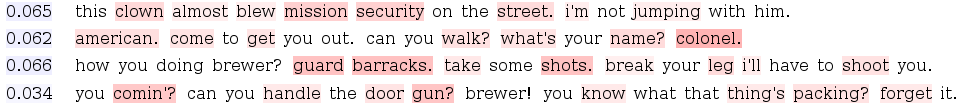
\includegraphics[scale=0.43]{pics/military.png}
   \caption{\textit{profession}: military personnel}
   \label{fig:att-profession}
 \end{subfigure}
 \\[8pt]
 \begin{subfigure}{.9\textwidth}
   \centering
   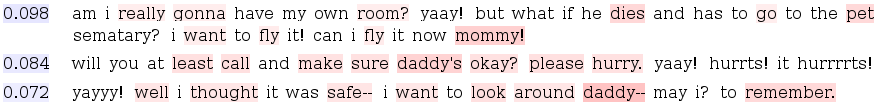
\includegraphics[scale=0.43]{pics/child.png}
   \caption{\textit{age} (category): child}
   \label{fig:att-age}
 \end{subfigure}
\vspace*{-0.3cm}
\caption{Attention visualization for \textit{profession} and \textit{age} attributes on MovieChAtt.}
\label{fig:att-profession-age}
\end{figure*}

\begin{figure*}[th!]
 \centering
 \begin{subfigure}{.9\textwidth}
   \centering
   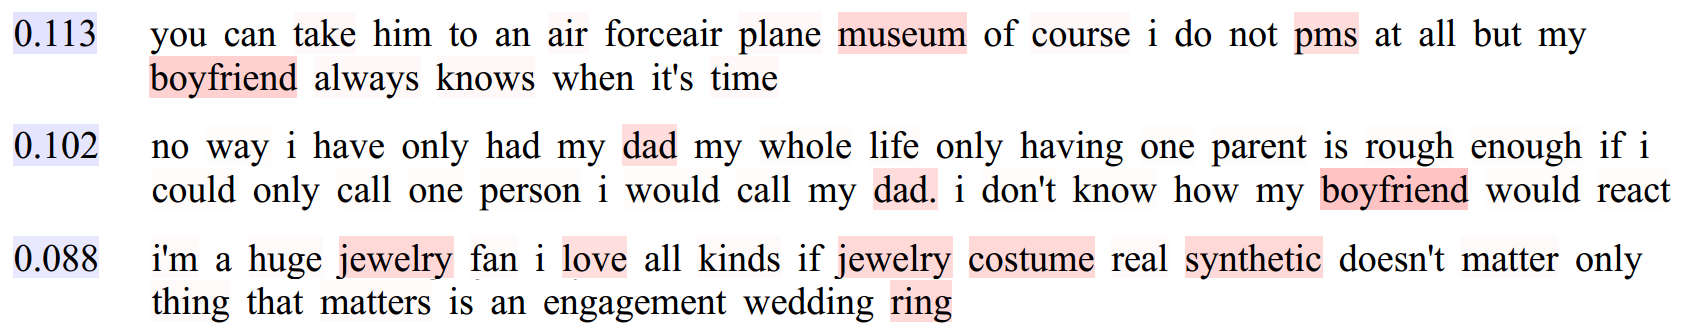
\includegraphics[scale=0.17]{pics/gender_att.png}
   \caption{\textit{gender}: female}
   \label{fig:att-gender}
 \end{subfigure}
 \\[8pt]
 \begin{subfigure}{.9\textwidth}
   \centering
   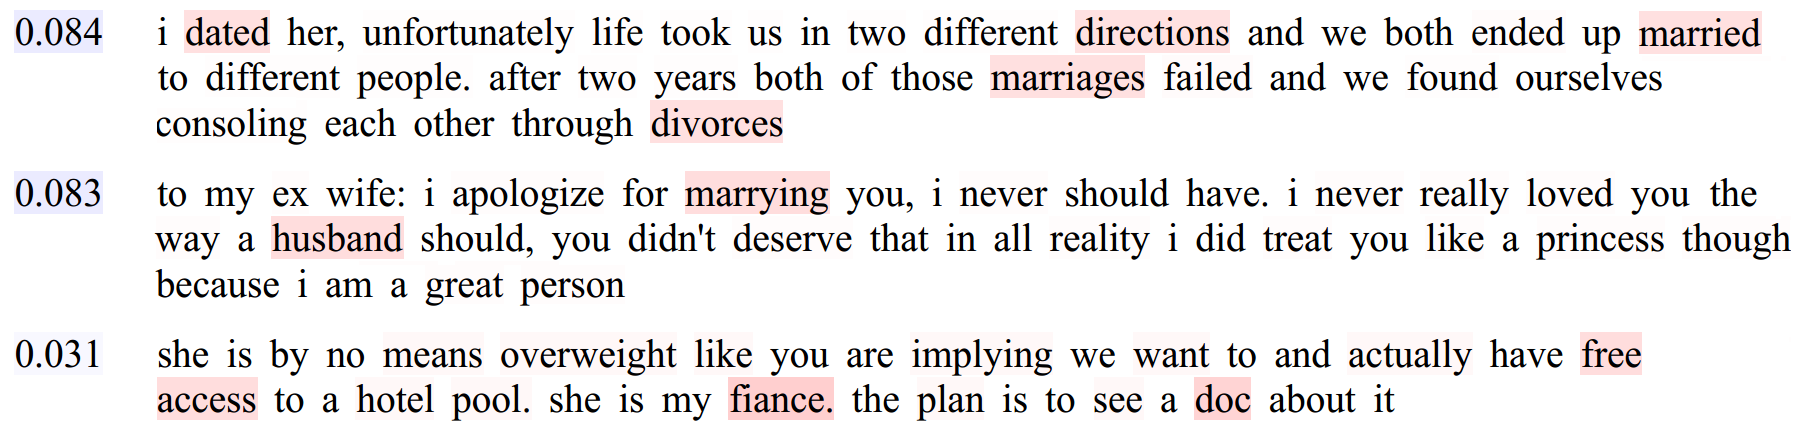
\includegraphics[scale=0.17]{pics/family_att.png}
   \caption{\textit{family status}: married}
   \label{fig:att-family}
 \end{subfigure}
\vspace*{-0.3cm}
\caption{Attention visualization for \textit{gender} and \textit{family status} attributes on RedDust.}
\label{fig:att-gender-family}
\end{figure*}


\subsection{Case study on attention weights}

In order to illustrate the types of terms the models are looking for, we display \method{2attn}'s term and utterance weights for 
\textit{profession} and \textit{age} attributes (on the MovieChAtt dataset) in Figure \ref{fig:att-profession-age}, as well as \textit{gender} and \textit{family status} attributes (on RedDust) in Figure \ref{fig:att-gender-family}.
While \method{2attn} is 
%sometimes
often outperformed by \method{CNN-attn}, this model is more interpretable because individual terms are considered in isolation.
%Note that all these dialogue snippets come from the specific
%datasets in our experiments, partly from fictional
%conversations.
%Some are skewed and biased, and not representative
%for the envisioned downstream applications.

When predicting \textit{military personnel} as the \textit{profession} (Figure \ref{fig:att-profession}), the model focuses on military terms such as \textit{mission}, \textit{guard}, \textit{barracks}, and \textit{colonel}.
When predicting \textit{child} as the \textit{age category} (Figure \ref{fig:att-age}), on the other hand, the model focuses on terms a child is likely to use, such as \textit{pet}, \textit{mommy}, and \textit{daddy}.
According to Reddit posts, \textit{female} gender is suggested by terms such as \textit{boyfriend}, \textit{pms} and \textit{jewelry} (Figure \ref{fig:att-gender}). Meanwhile, \textit{married} users were identified through terms such as \textit{dated}, \textit{fiance} and \textit{divorces}, along with obvious terms like \textit{marrying} and \textit{marriages} (Figure \ref{fig:att-family}). 
These examples illustrate how the model is able to infer a speaker's attribute by aggregating signals across utterances.

In addition to looking at specific utterances, we investigated which terms the model is strongly associating with a specific attribute. To do so, we computed attribute value probabilities for each term in the corpus, and kept the top terms for each attribute value. The results using \method{2attn} are shown in Table \ref{tab6}, which is divided into words that appear informative (top section) and words that do not (bottom section). In the case of informative words, there is a clear relationship between the words and the corresponding profession. 
Many of the uninformative words appear to be movie-specific, such as names (e.g., xavier, leonard) and terms related to a \textit{waiter's} role in a specific movie (e.g., rape, stalkers). Reducing the impact of setting-specific signals like this is one direction for future work.

\begin{table}[t]
\centering
\small
%\begin{adjustbox}{width=0.475\textwidth,center}
\begin{tabular}{@{}l@{\hskip 0.5\tabcolsep}l@{}}
\toprule
\textbf{profession} & \textbf{significant words} \\
\midrule
\textit{scientist} & characteristics, theory, mathematical, species, changes \\
\textit{politician} & governors, senate, secretary, reporters, president \\
\textit{detective} & motel, spotted, van, suitcase, parked \\
\textit{military personnel} & captured, firepower, guard, soldiers, attack \\
\midrule
\textit{student} & playing, really, emotional, definitely, unbelievable \\
\textit{photographer} & xavier, leonard, collins, cockatoo, burke \\
\textit{waiter} & rape, stalkers, murdered, overheard, bothering \\
\bottomrule
\end{tabular}
%\end{adjustbox}
\caption{Top-5 words from \method{2attn} characterizing each profession.
}
\label{tab6}
\end{table}

\vspace{-5pt}
\subsection{Insights on transfer learning}

To investigate the robustness of our trained HAMs,
we tested the best performing models (i.e., \method{2attn} and \method{CNN-attn})
on a transfer learning task between our datasets. 
Specifically, we leveraged user-generated social media text (RedDust posts) available in abundance to train the models and subsequently performing inference on the speech-based dialogues (MovieChAtt and PersonaChat). 
We report the results in Tables \ref{tab:transfer-learning-reddit-moviechatt} and \ref{tab:transfer-learning-reddit-personachat} respectively.

While the scores on PersonaChat are low compared to those in Tables \ref{tab:model-comparison-gender}, \ref{tab:model-comparison-profession} and \ref{tab:model-comparison-family}, the HAMs' performance on MovieChAtt is often comparable with the baselines' performance in Tables \ref{tab:model-comparison-gender}, \ref{tab:model-comparison-profession}, \ref{tab:model-comparison-age} and \ref{tab:model-comparison-family}.
This difference may be caused by the fact that PersonaChat is a smaller, more synthetic dataset, as discussed in Section \ref{findings}.

On MovieChAtt with the \textit{profession} attribute, both HAMs match the performance of all six baselines in terms of macro MRR. Similarly, \method{2attn} matches the performance of five of the six baselines on the \textit{gender} attribute (accuracy), and \method{CNN-attn} matches the performance of four of the six baselines on the \textit{age} attribute (macro MRR). The methods do not perform as well in terms of micro MRR, which may be due to the substantially different attribute value distributions between datasets.
Particularly for the \textit{profession} attribute, the lower performance can be explained by missing training instances  for certain professions in the RedDust dataset, such as \textit{astronaut} or \textit{monarch}. 
Improving HAMs' transfer learning performance is a direction for future work.


\begin{table}[t]
\centering
\small
\begin{adjustbox}{width=0.9\textwidth,center}
\begin{tabular}{@{}lc@{}cc@{\hskip 1\tabcolsep}cc@{}c@{}}
\toprule
\multirow{3}{*}{\textbf{Models}} & \multicolumn{2}{c}{\textbf{profession}\vspace{3pt}} & \multicolumn{2}{c}{\textbf{gender}} & \multicolumn{2}{c}{\textbf{age}} \\
\cmidrule(lr){2-3} \cmidrule(lr){4-5} \cmidrule(lr){6-7}
 & \multicolumn{1}{c}{MRR} & \multicolumn{1}{c}{\multirow{2}{*}{AUROC}} & \multicolumn{1}{c}{\multirow{2}{*}{Acc}} & \multicolumn{1}{c}{\multirow{2}{*}{AUROC}}  & \multicolumn{1}{c}{MRR} & \multicolumn{1}{c}{\multirow{2}{*}{AUROC}}  \\
 & \multicolumn{1}{c}{micro / macro} & &  & & \multicolumn{1}{c}{micro / macro} & \\
\midrule
\Tstrut \method{CNN-attn}     & 0.19 / 0.18 & 0.58 & 0.56 & 0.58 & \textbf{0.57} / \textbf{0.54} & \textbf{0.69} \\ 
\method{2attn}                & \textbf{0.21} / \textbf{0.21} & \textbf{0.67} & \textbf{0.61} & \textbf{0.64} & 0.45 / 0.41 & 0.45 \\
\bottomrule
\end{tabular}
\end{adjustbox}
\caption{Transfer learning performance of pre-trained RedDust models on MovieChAtt.}
\label{tab:transfer-learning-reddit-moviechatt}
\end{table}



\begin{table}[t]
\centering
\small
%\begin{adjustbox}{width=0.475\textwidth,center}
\begin{tabular}{@{}lcccccc@{}}
\toprule
\multirow{3}{*}{\textbf{Models}} & \multicolumn{2}{c}{\textbf{profession}\vspace{3pt}} & \multicolumn{2}{c}{\textbf{gender}} & \multicolumn{2}{c}{\textbf{family status}} \\
\cmidrule(lr){2-3} \cmidrule(lr){4-5} \cmidrule(lr){6-7} 
 & \multicolumn{1}{c}{MRR} & \multicolumn{1}{c}{\multirow{2}{*}{AUROC}} & \multicolumn{1}{c}{\multirow{2}{*}{Acc}} & \multicolumn{1}{c}{\multirow{2}{*}{AUROC}}  & \multicolumn{1}{c}{\multirow{2}{*}{Acc}} & \multicolumn{1}{c}{\multirow{2}{*}{AUROC}} \\
 & \multicolumn{1}{c}{micro / macro} &  &  &  &  & \\
\midrule
\Tstrut \method{CNN-attn}     & 0.20 / 0.16 & 0.58 & \textbf{0.52} & 0.50 & \textbf{0.74} & \textbf{0.74} \\
\method{2attn}                & \textbf{0.21} / \textbf{0.18} & \textbf{0.71} & 0.51 & \textbf{0.54} & 0.62 & 0.64 \\
\bottomrule
\end{tabular}
%\end{adjustbox}
\caption{Transfer learning performance of pre-trained RedDust models on PersonaChat.}
\label{tab:transfer-learning-reddit-personachat}
\end{table}

\subsection{Profession misclassification study}
In this section we investigate common misclassifications on the MovieChAtt dataset for the \textit{profession} attribute, which is the most challenging attribute with the most possible values.
A confusion matrix for \method{2attn} is shown in Figure \ref{matrix}.
Dotted lines indicate several
interesting misclassifications: \textit{policemen} are often confused with \textit{detectives} and \textit{special agents} (red line); \textit{scientists} are confused with \textit{astronauts} (yellow line), because sci-fi films often feature characters who arguably serve in both roles; and a \textit{child} is often labeled as a \textit{student} or a \textit{housewife} (green line) because they sometimes use similar terms (e.g., `school' is used by both children and students, and `mommy' is used by both children and housewives).
Finally, 
many occupations are confused with \textit{criminal}, which is the most common profession in MovieChAtt.


\begin{figure}[t]
\centering
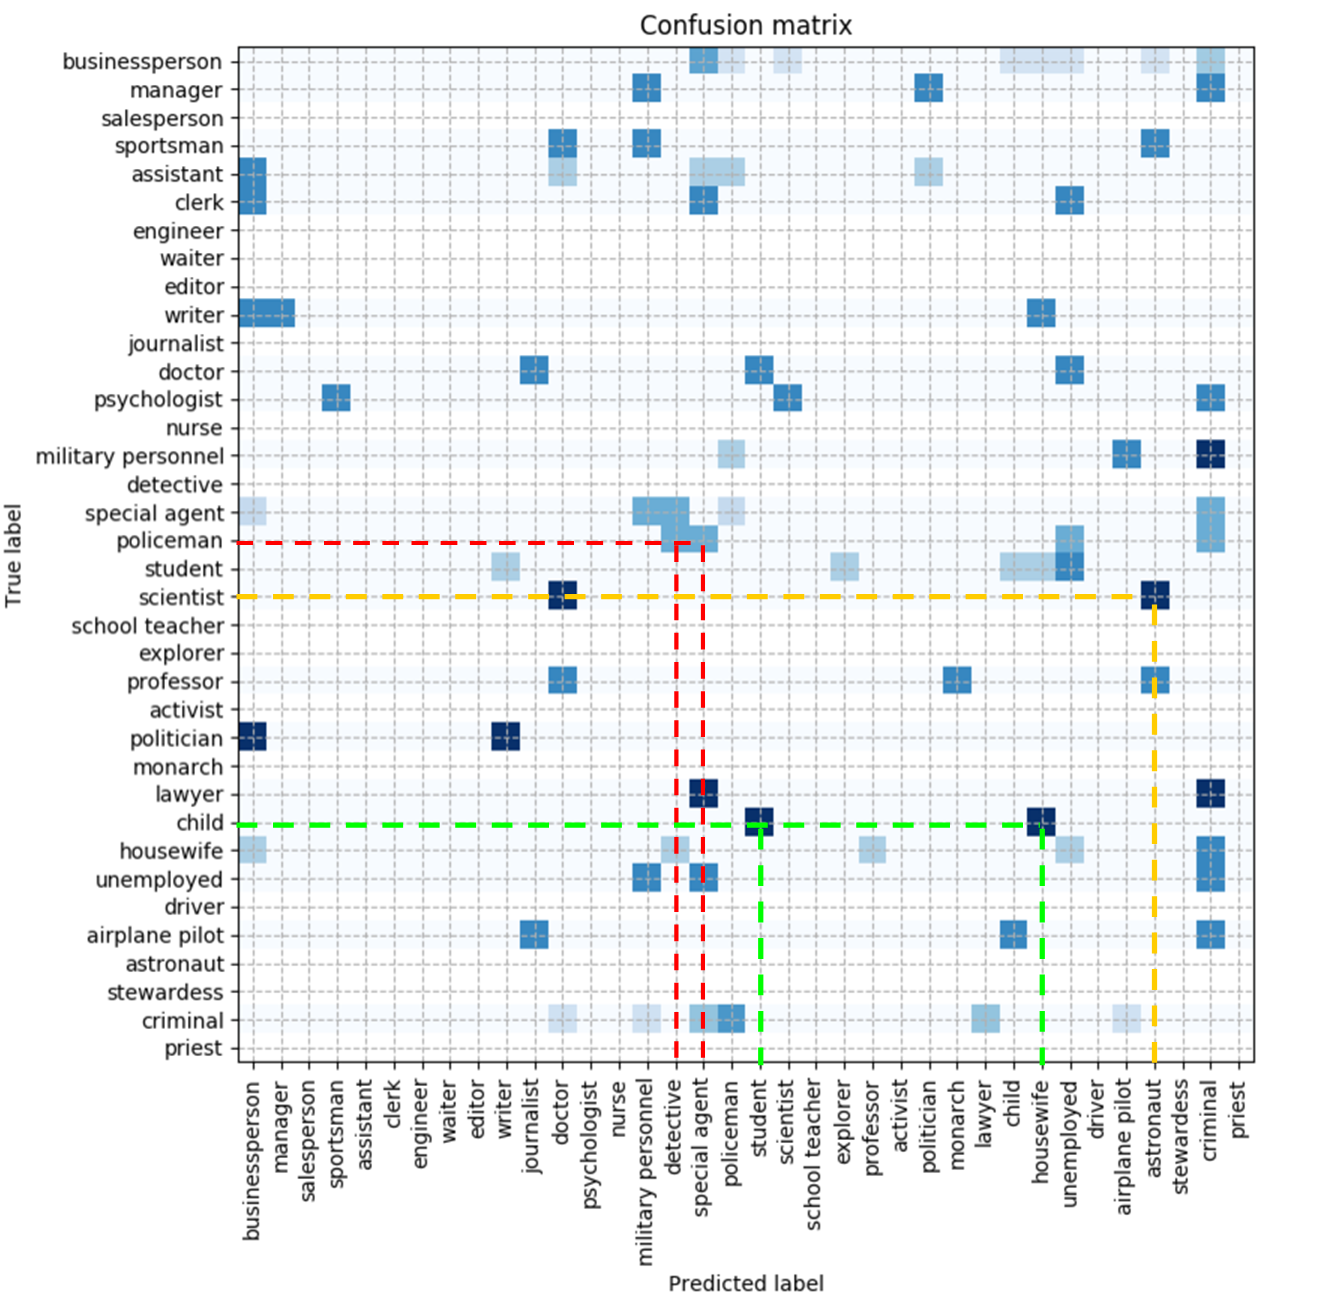
\includegraphics[width=0.7\textwidth]{pics/conf_new.png}
\vspace*{-0.3cm}
\caption{Confusion matrix computed with \method{2attn}. True positives are not shown. Darker squares indicate more misclassifications.}
\label{matrix}
\end{figure}



%%%%%
% Transfer learning confusion matrix (was in original HAM paper)
%
%To further compare the performance of the model on direct and transfer learning tasks we computed the confusion matrix for \method{2attn} trained on the Reddit dataset and using MovieChAtt as the test corpus. Interesting misclassifications include the following: artistic professions (\textit{actor}, \textit{painter}, \textit{musician}, \textit{director}) are often mixed up (red lines); \textit{banker} is confused with \textit{manager} (green lines); \textit{policeman} and \textit{airplane pilot} are confused with \textit{military personnel} (purple lines); and \textit{stewardess} is often confused with \textit{nurse} as they both are related to caring and serving tasks (yellow line).

%\begin{figure}[t]
%\centering
%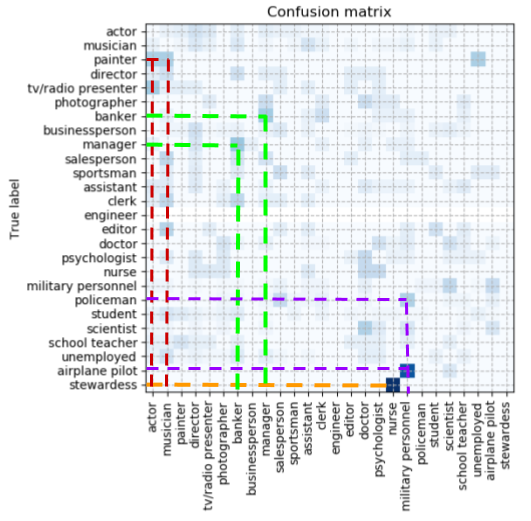
\includegraphics[width=0.75\textwidth]{pics/conf_transfer_crop.png}
%\vspace*{-0.3cm}
%\caption{Confusion matrix of Reddit$_{\text{train}}$ $\rightarrow$ %MovieChAtt$_{\text{test}}$ computed with \method{2attn}. True positives are not shown. %Darker squares indicate more misclassifications.}
%\label{matrix-reddit}
%\end{figure}

